% Supplementary Material for FidelityNO
\documentclass[10pt]{article}
\usepackage[T1]{fontenc}
\usepackage{lmodern}
\usepackage[utf8]{inputenc}
\usepackage[letterpaper,margin=1in]{geometry}
\usepackage{amsmath,amssymb,booktabs,graphicx,xcolor,hyperref,cleveref}
\graphicspath{{figures/}}
\renewcommand{\thesection}{S\arabic{section}}
\renewcommand{\thetable}{S\arabic{table}}
\renewcommand{\thefigure}{S\arabic{figure}}

\title{\textbf{Supplementary Material}}
\author{}
\date{}

\begin{document}
\maketitle
\noindent\textbf{Associated article:} Information-limited fidelity estimation of composed quantum channels: when to compose, measure, or learn.

\medskip
\noindent This supplement reports oracle verification, calibration diagnostics, sample-complexity results, ablations, length-shift analyses, representation ambiguity, measurement-conditioned fusion, readout-noise robustness, adaptive shot allocation, and ranking utility. All numbers are reproducible from the code described in the Data and Code Availability statements of the main paper.


%%%% BEGIN flattened: supp/S1_oracle.tex
\section{Oracle ground-truth verification}
\label{supp:oracle}

For the Markovian regimes, ground-truth entanglement fidelity $F_{\mathrm{e}}$ follows from exact channel composition and the closed-form identity-target formula. Collision labels use exact joint propagation of the system and bath. Bath retention between steps is set by $\eta$. We verify three properties of the Markovian pipeline.

\paragraph*{Associativity of Choi composition.}
We draw 2000 random channel triples $\Lambda_a, \Lambda_b, \Lambda_c$. Half use $d=2$ and half use $d=4$. We compare the two orderings $(\Lambda_a \star \Lambda_b) \star \Lambda_c$ and $\Lambda_a \star (\Lambda_b \star \Lambda_c)$. The maximum elementwise discrepancy is below $2\times10^{-13}$, which is at the numerical floor. The corresponding $F_{\mathrm{e}}$ values agree within $10^{-10}$. The released test suite includes this check.

\paragraph*{Independent simulator check.}
For $1{,}024$ Markovian sequences of mixed amplitude-damping, depolarising, and phase-damping channels with lengths $L \in \{2, 4, 8, 16, 24\}$ we compare our $F_{\mathrm{e}}$ against the value obtained by reconstructing the same superoperators with QuTiP and using its process-fidelity routine. The maximum discrepancy is $2.4 \times 10^{-8}$, the mean is $4.3 \times 10^{-9}$, and the median is $1.1 \times 10^{-15}$ (i.e.~most pairs agree to floating-point precision). This check provides an independent validation of the composition pipeline. The corresponding unit test uses 256 random sequences and gives identical statistics to within seed noise.

\paragraph*{CPTP sanity at every channel.}
Every channel produced by the channel libraries passes a CPTP test that checks (i) Choi positive semi-definiteness via Cholesky with tolerance $10^{-9}$, (ii) trace preservation $\mathrm{Tr}_{\mathrm{out}}\,J(\Lambda) = I$ to the same tolerance. The test runs as part of the standard validation suite and is required to succeed before any data-generation script is run.
%%%% END flattened: supp/S1_oracle.tex


%%%% BEGIN flattened: supp/S2_calibration.tex
\section{Extended calibration diagnostics}
\label{supp:calibration}

Table~\ref{tab:supp_calibration} reports distributional metrics for the collision regime. The legacy \texttt{family\_ood} filename refers to the high-retention interval $\eta\in[0.85,0.99]$. The collision family is shared with training. Two figures provide additional diagnostics. The first compares expected calibration error (ECE) before and after split-conformal recalibration on ID. The second gives reliability diagrams for ID and the $n=48$ length-OOD endpoint.

\begin{figure}[h]
\centering
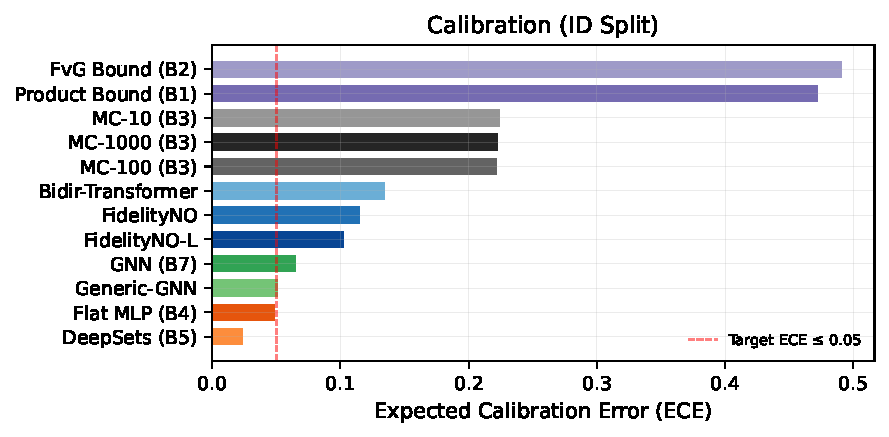
\includegraphics[width=0.86\linewidth]{calibration_ece.pdf}
\caption{Expected calibration error before and after split-conformal recalibration on the in-distribution test split. The quantile-head neural surrogates improve after recalibration, with FidelityNO reaching the low-error region used in the main-paper comparison.}
\label{fig:supp_ece}
\end{figure}

\begin{figure}[h]
\centering
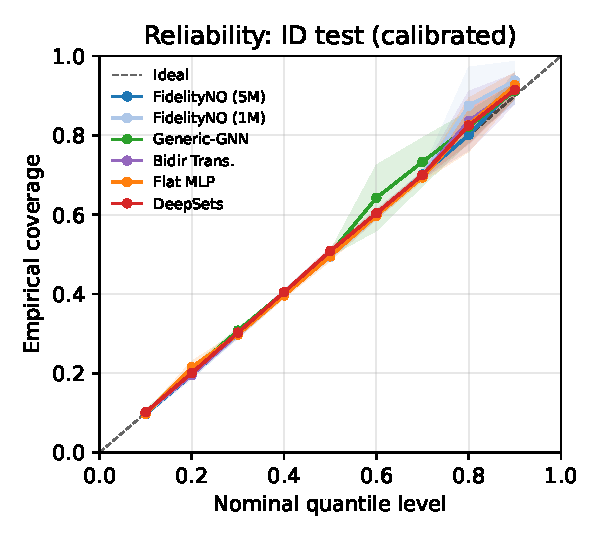
\includegraphics[width=0.48\linewidth]{reliability_id.pdf}\hfill
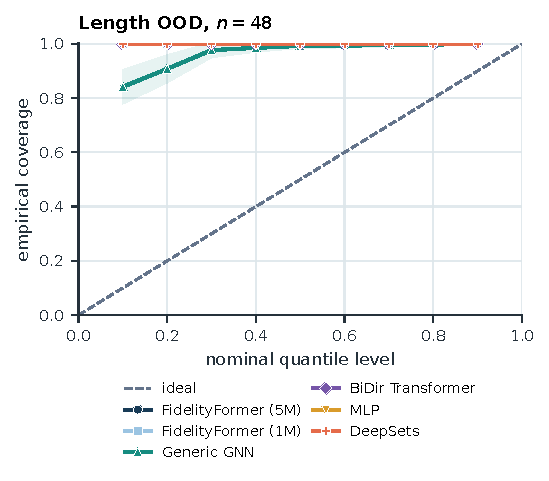
\includegraphics[width=0.48\linewidth]{reliability_len48.pdf}
\caption{Reliability diagrams after split-conformal recalibration. The left panel shows the in-distribution split, where the neural surrogates follow the diagonal and agree with the low expected calibration errors in Table~\ref{tab:supp_calibration}. The right panel shows the length out-of-distribution split at $n=48$. All methods become conservative because conformal offsets fitted on $n\le16$ overstate uncertainty under this length shift.}
\label{fig:supp_reliability}
\end{figure}

\begin{table}[h]
\centering
\caption{Extended pre-affine distribution metrics for FidelityNO on the collision regime. Additive conformal offsets are fitted on \texttt{calib.npz}. Mean absolute error gives the raw point error before the labelled out-of-distribution affine correction used in the main collision table. Results cover five seeds and 1024 sequences per split.}
\label{tab:supp_calibration}
\begin{tabular}{lcccc}
\toprule
Split & MAE & Pinball & CRPS & ECE \\
\midrule
\texttt{id\_test} & 0.025 & 0.009 & 0.018 & \textbf{0.004} \\
\texttt{length\_ood} & 0.138 & 0.060 & 0.119 & 0.394 \\
\texttt{family\_ood} & 0.383 & 0.179 & 0.359 & 0.500 \\
\bottomrule
\end{tabular}
\end{table}

\paragraph*{Calibration interpretation.}
The ID ECE is $0.004$, below the threshold of $0.05$ used in our analysis. ECE rises to $0.39$ and $0.50$ on the two OOD splits. Conformal offsets fitted on ID transfer poorly across these shifts. FidelityNO+cal uses a separate affine correction fitted on labelled OOD data. The MAE column is measured before that correction and matches the raw FidelityNO result up to rounding. Synthetic OOD labels come from exact joint propagation of the system and bath. A hardware experiment would obtain them through measurement or characterisation. Section~\ref{supp:sample_complexity} counts the cost of finite-shot DFE labels.

\paragraph*{Reliability diagram.}
The released figures show empirical coverage for each predicted quantile. ID curves follow the diagonal closely. On OOD data, lower quantiles tend to over-cover and upper quantiles tend to under-cover. This pattern agrees with the mean shift measured in the affine-recalibration analysis.
%%%% END flattened: supp/S2_calibration.tex


%%%% BEGIN flattened: supp/S3_sample_complexity.tex
\section{Corrected DFE and calibration-cost audit}
\label{supp:sample_complexity}

The first DFE implementation sampled Pauli settings with replacement and assigned 200 shots to each draw. This estimator is unbiased and has extra protocol variance for the single-qubit identity target, whose relevance support contains four Pauli settings. The revised implementation enumerates the support, allocates a fixed total budget across settings, and samples exact binomial $\{+1,-1\}$ outcomes. Table~\ref{tab:supp_dfe} reports the low-shot curve on 1024 memory-strength-OOD sequences.

\begin{table}[h]
\centering
\caption{Stratified Direct Fidelity Estimation on the collision memory-strength out-of-distribution split. The estimator acts on the true composed process.}
\label{tab:supp_dfe}
\begin{tabular}{rrr}
\toprule
total shots/sequence & MAE in $F_{\mathrm e}$ & RMSE in $F_{\mathrm e}$ \\
\midrule
4 & 0.282 & 0.328 \\
8 & 0.183 & 0.227 \\
16 & 0.135 & 0.167 \\
32 & 0.092 & 0.113 \\
64 & 0.065 & 0.082 \\
128 & 0.044 & 0.055 \\
256 & 0.032 & 0.041 \\
512 & 0.023 & 0.029 \\
1024 & 0.016 & 0.020 \\
\bottomrule
\end{tabular}
\end{table}

At 2000 shots per sequence, stratified DFE gives MAE $0.0069$ on ID, $0.0112$ on length OOD, and $0.0116$ on memory-strength OOD. These values replace the earlier with-replacement curve. The bidirectional model with $N_{\mathrm{cal}}=64$ reaches MAE about $0.087$. Stratified DFE approaches this error near 32 shots per query and gives a lower error at 64 shots.

\paragraph*{Finite-shot calibration labels.}
The main text also audits the one-time cost of labelled OOD calibration. We estimate every calibration label by stratified DFE, fit the same affine map, and evaluate against exact held-out labels. Table~\ref{tab:supp_noisy_cal} pools five bidirectional checkpoints and five independent measurement repetitions. With 64 labels, 64 shots per label are enough for the calibration-noise penalty to be negligible.

\begin{table}[h]
\centering
\caption{Bidirectional model with $N_{\mathrm{cal}}=64$ finite-shot calibration labels. The exact-label reference mean absolute error is $0.087$.}
\label{tab:supp_noisy_cal}
\begin{tabular}{rrc}
\toprule
shots/label & total offline shots & test MAE (mean $\pm$ std) \\
\midrule
16 & 1024 & $0.092\pm0.007$ \\
32 & 2048 & $0.091\pm0.006$ \\
64 & 4096 & $0.087\pm0.003$ \\
128 & 8192 & $0.085\pm0.001$ \\
512 & 32768 & $0.086\pm0.001$ \\
\bottomrule
\end{tabular}
\end{table}

\paragraph*{Reproduction protocol.}
Run \texttt{scripts/eval\_dfe.py} with \texttt{--strategy stratified --M 1} and the total-shot values above. The companion noisy-calibration evaluation script reproduces the calibration audit. Both scripts record the seed, evaluated sample count, and total shot budget in CSV output.

\paragraph*{Marginal Monte Carlo.}
Classical Kraus-path sampling uses reset-bath marginals and has no observation of the retained bath. Increasing the path count reduces sampling variance around the marginal-composed process. The bias from memory strength remains.
%%%% END flattened: supp/S3_sample_complexity.tex


%%%% BEGIN flattened: supp/S4_ablations.tex
\section{Additional ablations}
\label{supp:ablations}

We test the auxiliary physics-consistency weight, the distribution head, and the channel representation. The main paper reports the comparison between causal and bidirectional attention. All variants use the same collision data, optimiser, and curriculum. The default model uses five seeds and each ablation uses three. Every split contains 1024 sequences.

\paragraph*{Auxiliary physics-consistency loss.}
The default model uses an auxiliary head predicting the purity and trace of the composed Choi, with weight $\lambda_{\mathrm{aux}} = 0.1$. Table~\ref{tab:supp_ablation_aux} reports collision-regime raw (uncalibrated) MAE with this loss off, default, and at heavier weight.

\begin{table}[h]
\centering
\caption{Auxiliary physics-consistency loss ablation. The table reports pooled raw mean absolute error on the collision regime and in-distribution expected calibration error.}
\label{tab:supp_ablation_aux}
\begin{tabular}{lccccc}
\toprule
$\lambda_{\mathrm{aux}}$ & seeds & \texttt{id\_test} & \texttt{length\_ood} & \texttt{family\_ood} & ECE (\texttt{id\_test}) \\
\midrule
$0.0$ & 3 & $0.0240$ & $0.1390$ & $0.3867$ & $0.021$ \\
$0.1$ (default) & 5 & $0.0247$ & $0.1377$ & $0.3869$ & $0.018$ \\
$0.5$ & 3 & $0.0238$ & $0.1384$ & $0.3881$ & $0.020$ \\
\bottomrule
\end{tabular}
\end{table}

The three auxiliary-loss settings differ by at most $0.0014$ across the collision splits, which lies within seed variation. We keep $\lambda_{\mathrm{aux}}=0.1$ for consistency with the earlier runs. Removing the auxiliary loss produces similar point-prediction MAE.

\paragraph*{Quantile head versus Gaussian head.}
Table~\ref{tab:supp_ablation_head} compares the primary 9-quantile pinball head against a parametric truncated-Gaussian head trained with NLL.

\begin{table}[h]
\centering
\caption{Distribution-head ablation. Pooled raw mean absolute error and in-distribution expected calibration error on the collision regime.}
\label{tab:supp_ablation_head}
\begin{tabular}{lccccc}
\toprule
Head & seeds & \texttt{id\_test} & \texttt{length\_ood} & \texttt{family\_ood} & ECE (\texttt{id\_test}) \\
\midrule
Quantile (default) & 5 & $0.0247$ & $0.1377$ & $0.3869$ & $0.018$ \\
Gaussian & 3 & $0.0248$ & $0.1369$ & $0.3876$ & $0.039$ \\
\bottomrule
\end{tabular}
\end{table}

The two heads give similar point-prediction MAE. Their calibration differs on ID. The Gaussian head has ECE $0.039$, compared with $0.018$ for the quantile head. We use the quantile head for its lower calibration error.

\paragraph*{Choi versus Pauli-transfer-matrix encoder.}
We also test a Pauli-transfer-matrix (PTM) encoder. For a single-qubit channel, the Choi feature has 32 real and imaginary entries. The PTM has 16 real entries given by $R_{ij}=(1/d)\mathrm{Tr}[P_i\Lambda(P_j)]$. We zero-pad the PTM to the same input width. A precomputed Choi-to-PTM tensor performs the conversion in one contraction. Table~\ref{tab:supp_ablation_encoder} reports the collision MAE for both encoders.

\begin{table}[h]
\centering
\caption{Channel-encoder ablation: Choi versus Pauli transfer matrix. All other architecture choices are identical.}
\label{tab:supp_ablation_encoder}
\begin{tabular}{lccccc}
\toprule
Encoder & seeds & \texttt{id\_test} & \texttt{length\_ood} & \texttt{family\_ood} & ECE (\texttt{id\_test}) \\
\midrule
Choi (default) & 5 & $0.0247$ & $0.1377$ & $0.3869$ & $0.018$ \\
PTM & 3 & $0.0247$ & $0.1356$ & $0.3863$ & $0.018$ \\
\bottomrule
\end{tabular}
\end{table}

For $d=2$, the two encoders differ by at most $0.0021$ across all splits and metrics. This difference lies within seed variation. We use Choi throughout the paper so that the representation stays unchanged between the single-qubit and $d=4$ experiments. At $d=4$, the PTM contains 256 real values per channel and the real-imaginary Choi feature contains 512. The single-qubit ablation shows similar accuracy and calibration for the two choices. The released implementation documents the PTM encoder, and the reported $d=4$ runs use Choi.

\paragraph*{Interpretation of the ablations.}
The collision regime contains bath-mediated correlations across time steps. A causal transformer processes channel tokens, and the OOD affine fit corrects the deployment shift. Within this configuration, the auxiliary loss and the channel representation have little effect on MAE. The distribution head mainly affects calibration.
%%%% END flattened: supp/S4_ablations.tex


%%%% BEGIN flattened: supp/S5_length_ood.tex
\section{Length-OOD diagnostics}
\label{supp:length_ood}

The main paper reports pooled affine-recalibrated MAE of $0.077$ for length OOD with $L\in\{24,32,48\}$. The following diagnostic reports each length before the pooled affine correction and shows how the raw bias changes with sequence length.

\begin{table}[h]
\centering
\caption{Pre-affine length-by-length diagnostic for the collision regime. Results cover five seeds and 1024 sequences per length. The legacy sampling table used a different subset. Corrected pooled sampling results appear in the main text and Sec.~\ref{supp:sample_complexity}.}
\label{tab:supp_length_breakdown}
\begin{tabular}{lcc}
\toprule
$L$ & FidelityFormer raw & product approximation \\
\midrule
$24$ & $0.082$ & $0.061$ \\
$32$ & $0.130$ & $0.080$ \\
$48$ & $0.209$ & $0.114$ \\
\bottomrule
\end{tabular}
\end{table}

\paragraph*{Length-dependent error trends.}
The table reports length dependence before pooled affine OOD recalibration. Both predictors degrade as $L$ grows, and the raw learned predictor has the larger bias at $L=48$. The pooled affine correction reduces the overall length-OOD MAE to $0.077$. The per-length values show that much of the raw bias comes from the longest sequences. A separate affine fit for each length reduces the $L=48$ error further and requires labelled examples for every deployment length. The reported configuration uses one pooled fit and one shared label budget.

\paragraph*{Per-seed (a, b) coefficients.}
\Cref{tab:supp_per_seed_ab} reports the affine coefficients for each \texttt{family\_ood} seed. The slope and intercept have standard deviations $0.091$ and $0.081$. The post-calibration MAE has standard deviation $0.0013$. Different coefficient pairs give similar predictive error.

\begin{table}[h]
\centering
\caption{Affine recalibration coefficients $(a, b)$ on \texttt{family\_ood}, per seed. The linear fit $F_{\mathrm{cal}} = a \cdot F_{\mathrm{raw}} + b$ uses a labelled, held-out 10\% out-of-distribution calibration set.}
\label{tab:supp_per_seed_ab}
\begin{tabular}{ccccc}
\toprule
seed & $a$ & $b$ & raw MAE & corrected MAE \\
\midrule
$0$ & $2.845$ & $-1.916$ & $0.387$ & $0.0952$ \\
$1$ & $2.822$ & $-1.896$ & $0.386$ & $0.0949$ \\
$2$ & $2.918$ & $-1.980$ & $0.387$ & $0.0937$ \\
$3$ & $3.026$ & $-2.080$ & $0.388$ & $0.0954$ \\
$4$ & $3.003$ & $-2.052$ & $0.387$ & $0.0923$ \\
\midrule
mean & $2.923$ & $-1.985$ & $0.387$ & $0.0943$ \\
std & $0.091$ & $0.081$ & $0.0008$ & $0.0013$ \\
\bottomrule
\end{tabular}
\end{table}
%%%% END flattened: supp/S5_length_ood.tex

\section{Representation ambiguity and measurement-conditioned fusion}
\label{supp:identifiability}

\subsection{Proof of the fibre-wise lower bound}
Fix an observed representation $x$ and choose $z,z'\in\mathcal A_\phi(x)$. Every estimator using only $x$ returns the same value $h(x)$ on both instances. The triangle inequality gives
\[
|F(z)-F(z')|\leq |F(z)-h(x)|+|h(x)-F(z')|.
\]
At least one term on the right is at least $|F(z)-F(z')|/2$. Taking the supremum over pairs proves Eq.~(5) of the main text. For absolute loss, the subgradient of $\mathbb E[|F-a|\mid x]$ changes sign at a conditional median. This establishes Eq.~(6). The minimax quantity applies to the worst case within each fibre. The Bayes quantity averages over fibres under a stated distribution.

\subsection{Counterfactual protocol and random-stream control}
We sample 2048 base collision sequences with lengths in $\{8,16,24\}$. For each base, we retain its couplings, frequencies, durations, bath initial state, and reset-bath marginal Choi sequence, then replay joint propagation at 15 equally spaced values in $\eta\in[0.85,0.99]$. This gives 30,720 physical labels grouped into 2048 exactly identical observable inputs. The maximum tensor difference within every group is zero in float32 storage. Diameter is the within-group maximum minus minimum. The empirical Bayes estimate is the mean absolute deviation from the within-group median under the uniform 15-point grid.

To exclude pseudorandom coupling, we also generate a fresh 4096-instance evaluation set using seed 20260807 for collision parameters and a separate seed 920260807 for $\eta$. Its label mean and standard deviation are 0.4472 and 0.1979. On this split, 64-label affine BiDir calibration gives MAE 0.0894, summary ridge 0.0977, exact-marginal affine 0.1101, and an oracle ridge that additionally observes $\eta$ 0.0800. These values reproduce the legacy split ordering without sharing a random stream.

\subsection{Independent exchange-coupled memory audit}
The second audit uses the step Hamiltonian
\begin{equation}
H_t=\frac{J_t}{2}(X_SX_B+Y_SY_B)
+\frac{\Delta_t}{2}Z_SZ_B
+\frac{\omega_t}{2}I_SZ_B.
\end{equation}
The exchange term and local bath-precession term do not commute. The reset state is $\rho_B=0.8|0\rangle\langle0|+0.2|1\rangle\langle1|$. We sample $J_t\in[0.08,0.25]$, $\Delta_t\in[0.02,0.12]$, $\omega_t\in[0.08,0.30]$, and collision duration $\tau_t\in[0.25,0.90]$. For each of 1024 base sequences, the same reset-bath marginals are replayed at 15 retention values in $[0.85,0.99]$. The parameter seed is 20260810.

\begin{table}[h]
\centering
\caption{Length-resolved ambiguity for the exchange-coupled audit.}
\label{tab:supp_exchange_audit}
\begin{tabular}{rrrrr}
\toprule
Length & inputs & mean diameter & mean minimax floor & Bayes MAE floor \\
\midrule
8  & 346 & 0.0617 & 0.0309 & 0.0164 \\
16 & 322 & 0.1000 & 0.0500 & 0.0269 \\
24 & 356 & 0.1372 & 0.0686 & 0.0307 \\
\midrule
All & 1024 & 0.1000 & 0.0500 & 0.0247 \\
\bottomrule
\end{tabular}
\end{table}

The maximum marginal-Choi change across the retention grid is zero. At $\eta=0$, joint propagation and exact marginal composition agree within $5.6\times10^{-16}$. Exact composition of the reset-bath marginals has mean absolute error $0.247$ over the high-memory grid. This value measures missing memory rather than numerical composition error.

\subsection{Full finite-label shot sweep}
Every finite-label run uses 64 calibration instances. Independent 64-shot stratified Direct Fidelity Estimation estimates provide their target labels. For each budget $B$, a separate $B$-shot outcome on every calibration instance fits $w_B$ in Eq.~(10). A third random stream generates the test measurements. Target labels and pilot features come from different outcomes. All methods use the same test indices and test Direct Fidelity Estimation outcomes. Neural entries aggregate five checkpoints and five measurement repeats. Other entries use five measurement repeats.

\begin{table}[h]
\centering
\caption{Full independent-random-stream shot sweep. Values give the mean and standard deviation of the mean absolute error. Offline shots for either hybrid are $4096+64B$.}
\label{tab:supp_hybrid_sweep}
\small
\begin{tabular}{rccc}
\toprule
$B$ & stratified DFE & BiDir hybrid & summary-ridge hybrid \\
\midrule
4   & $0.2755\pm0.0029$ & $0.0849\pm0.0043$ & $0.0946\pm0.0051$ \\
8   & $0.1856\pm0.0021$ & $0.0810\pm0.0025$ & $0.0868\pm0.0029$ \\
16  & $0.1299\pm0.0015$ & $0.0758\pm0.0039$ & $0.0805\pm0.0050$ \\
32  & $0.0909\pm0.0012$ & $0.0657\pm0.0019$ & $0.0683\pm0.0027$ \\
48  & $0.0743\pm0.0013$ & $0.0590\pm0.0014$ & $0.0605\pm0.0016$ \\
64  & $0.0641\pm0.0005$ & $0.0539\pm0.0012$ & $0.0557\pm0.0024$ \\
96  & $0.0525\pm0.0004$ & $0.0473\pm0.0011$ & $0.0485\pm0.0024$ \\
128 & $0.0455\pm0.0004$ & $0.0424\pm0.0016$ & $0.0438\pm0.0028$ \\
\bottomrule
\end{tabular}
\end{table}

The mean neural fusion weight rises from 0.071 at four shots to 0.783 at 128 shots. At low budgets, the model supplies most of the estimate because the pilot has high variance. As the pilot becomes more precise, DFE receives more weight. Exact-label and finite-label calibration give similar curves. At high budgets, all priors converge toward DFE. The largest difference between neural and ridge priors occurs at low and intermediate budgets.

\subsection{Symmetric readout-noise stress test}
We independently flip each sampled binary Pauli outcome with probability $p_r$. This attenuates the observed expectation by $1-2p_r$. The calibrated result divides each observed expectation by this factor. The inversion is left unclipped until the final fidelity estimate, so its finite-shot variance is retained. Offline target labels use the clean finite-shot protocol from the main experiment. The query and fusion-pilot outcomes contain the stated readout error.

\begin{table}[h]
\centering
\caption{MAE under symmetric readout error. DFE and hybrid entries use calibrated linear inversion. Hybrid values average five checkpoints and five measurement repeats.}
\label{tab:supp_readout}
\begin{tabular}{ccccc}
\toprule
$p_r$ & DFE-32 & hybrid-32 & DFE-64 & hybrid-64 \\
\midrule
0.00 & 0.0908 & 0.0650 & 0.0642 & 0.0533 \\
0.01 & 0.0949 & 0.0659 & 0.0670 & 0.0552 \\
0.03 & 0.1043 & 0.0697 & 0.0737 & 0.0598 \\
0.05 & 0.1128 & 0.0712 & 0.0807 & 0.0623 \\
\bottomrule
\end{tabular}
\end{table}

At $p_r=0.05$, leaving the readout error uncorrected gives MAE 0.1089 and 0.0823 for 32-shot and 64-shot DFE. The corrected values are 0.1128 and 0.0807. Linear inversion is unbiased before final clipping but increases variance, so it need not improve MAE at low shot counts. The hybrid changes its fitted measurement weight and improves after correction at both budgets. Its corresponding uncorrected errors are 0.0735 and 0.0660.

\subsection{Two-stage shot allocation}
Every query first receives an 8-shot stratified pilot. At average budget 32, half of the queries finish at 16 shots and half at 48. At average budget 64, the two levels are 32 and 96. The combined policy ranks queries by the sum of the fractional ranks of predictive interval width and prior-pilot disagreement. A random allocation with the same total budget is included as a control. Fusion weights are fitted separately for the two realised budgets.

\begin{table}[h]
\centering
\caption{Uniform and combined-score allocation for the neural hybrid. The interval is a paired two-way cluster bootstrap confidence interval over five checkpoints and five measurement repeats for adaptive minus uniform MAE.}
\label{tab:supp_adaptive}
\begin{tabular}{rrrrc}
\toprule
Average shots & allocation levels & uniform MAE & adaptive MAE & difference, 95\% CI \\
\midrule
32 & 16 / 48 & 0.0660 & 0.0648 & $-0.00116\;[-0.00312,0.00136]$ \\
64 & 32 / 96 & 0.0531 & 0.0543 & $\phantom{-}0.00113\;[-0.00035,0.00341]$ \\
\bottomrule
\end{tabular}
\end{table}

Both confidence intervals include zero. Random allocation is worse than uniform at both budgets. This experiment does not establish a general gain from query-adaptive allocation. The low-budget point estimate suggests a possible benefit, while the variance cost of reducing shots on other queries remains substantial.

\subsection{Zero-shot ranking utility}
We evaluate raw BiDir predictions before OOD affine correction. Across five checkpoints, Pearson correlation is $0.815\pm0.005$, Spearman correlation is $0.710\pm0.002$, and Kendall correlation is $0.534\pm0.002$. The predicted highest-fidelity 10\% set overlaps the true set by $0.858\pm0.004$. The lowest-fidelity 10\% overlap is $0.144\pm0.012$, compared with 0.10 in expectation for a random set. The uncalibrated predictor is useful for selecting high-fidelity candidates on this split. It gives little support for low-fidelity failure triage.


\end{document}
